\chapter{Project Results}
\label{chapter:project_results}
In the following chapter, the author will analyse the results obtained from the hardware and software developed in this thesis project. The author's first objective was running the \enquote{Hello World!} firmware with the \textit{VexRiscv} \acrshort{cpu}. Secondly, he tested the implementation of the interrupt routine software with the developed \acrshort{clint} hardware. Finally, the candidate successfully executed the minimal Linux \acrshort{os} in real hardware using the developed \acrlong{soc}.

All the results obtained in this thesis which communicate with the \acrshort{fpga} board or the \acrshort{soc} testbench, are executing the developed \textit{Console} program. The hardware components comprising the \acrshort{soc} differ in each section of this chapter. The author customises the \acrshort{soc} hardware depending on the software needs. Along this chapter, the developed \acrshort{soc} will be referenced as the \textit{IOb-SoC-Linux}.

In each step, the author studied the simulation with the different logic simulators and the memory resources needed to run the respective firmware. Furthermore, when running the \acrshort{soc} on the \acrshort{fpga} board he examined the required \acrshort{fpga} resources.

\section{System Running \enquote{Hello World!}}
\label{section:hello_world}
The \textit{IObundle} developers created the \enquote{Hello World!} firmware to test the functionality of the \textit{IOb-SoC} template. After the author implemented the \textit{VexRiscv} \acrshort{cpu} on the developed \acrshort{soc}, he executed a regression test to verify the correctness of the \acrshort{soc}. The regression test was the execution of the \enquote{Hello World!}, which was known to work correctly on the \textit{IOb-SoC}.

The \enquote{Hello World!} firmware is a program that prints a \enquote{Hello World!} message to the user, prints the value of $\pi$, which is a floating number, and tests file transferring between the \textit{Console} and \textit{IOb-SoC}. The alterations the author made to the \textit{IOb-SoC} hardware to obtain the results presented in this section was swapping the \acrshort{cpu} and removing the \textit{IOb-SoC} external memory L1 cache.

The firmware size dictates the minimal size of the memory on the \acrshort{soc}. The \textit{IOb-SoC-Linux} memory is 32 KB because the \enquote{Hello World!} program size is 23964 Bytes. The memory size should always be the closest upper bound power of two. 

\subsection{Execute in simulation}
The author simulated the \enquote{Hello World!} program using the \textit{Icarus} simulator and \textit{Verilator}. The \enquote{Hello World!} simulation allows the author to make a fair comparison between both logic simulators.

In figure \ref{fig:hello_sim}, the reader can see the expected output when executing the \enquote{Hello World!} firmware. In this example, the simulator executed the firmware using the internal memory of the \acrshort{soc} and considered that the firmware was already on the memory. Considering the firmware was already on the memory, allow the simulator not to execute the firmware transfer between the \textit{Console} and the testbench.

\begin{figure}[!ht]
    \centering
    \begin{subfigure}[b]{0.49\textwidth}
        \centering
        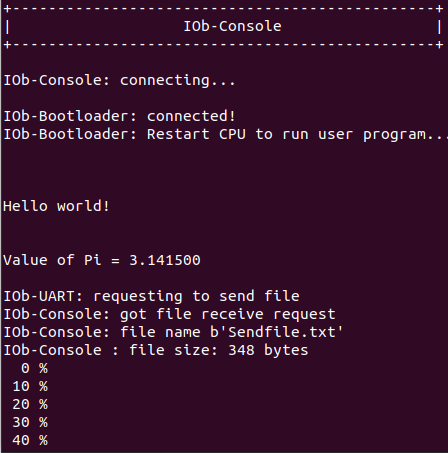
\includegraphics[width=\textwidth]{start_Hello_sim.png}
        \caption{Start of the \enquote{Hello World!} firmware.}
        \label{fig:start_hello_sim}
    \end{subfigure}
    \hfill
    \begin{subfigure}[b]{0.49\textwidth}
        \centering
        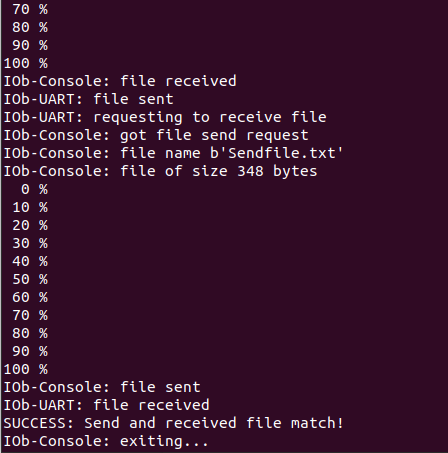
\includegraphics[width=\textwidth]{end_Hello_sim.png}
        \caption{End of the \enquote{Hello World!} firmware.}
        \label{fig:end_hello_sim}
    \end{subfigure}
    \caption{Running the \enquote{Hello World!} firmware in simulation.}
    \label{fig:hello_sim}
\end{figure}

Both open-source logic simulators are capable of executing the \enquote{Hello World!} program. The simulation is slower when the baud rate decreases or the memory size increases. The baud rate used in the simulation was 5000000. The baud rate is the number of bits per second transferred to the \acrshort{uart}. The author executed the simulations considering the system clock frequency 100MHz. The \acrshort{soc} always stores the bootloader in internal memory. The bootloader memory is 4KB ($2^12$). Since the bootloader binary is 1508 Bytes, 4KB is enough memory to store the bootloader program. The firmware, by default, is stored in the internal memory, and the memory size is 32KB ($2^15$). In table \ref{tab:hello_sim} the reader can see a timing comparison between the different logic simulators simulating the original \textit{IOb-SoC} and the developed \acrshort{soc}. The \enquote{INIT\_MEM} flag indicates whether the firmware is already loaded in the \acrshort{fpga} or if the \textit{Console} needs to transfer the firmware to the \acrshort{soc}, the user can set the flag to '1' or '0' respectively. The users can execute the simulations with or without external memory. Furthermore, the firmware can run in internal or external memory. The \enquote{make sim-test} command tests the different possible simulations.

\begin{table}[!ht]
    \centering
    \begin{tabular}{l|ll|ll|}
    \cline{2-5}
                                                           & \multicolumn{2}{l|}{\textit{IOb-SoC-Linux}} & \multicolumn{2}{l|}{\textit{IOb-SoC}}    \\ \hline
    \multicolumn{1}{|l|}{Command \textbackslash Simulator} & \multicolumn{1}{l|}{Icarus}  & Verilator & \multicolumn{1}{l|}{Icarus}  & Verilator \\ \hline
    \multicolumn{1}{|l|}{make sim-run INIT\_MEM=1}              & \multicolumn{1}{l|}{2m 26s}  & 0m 3s     & \multicolumn{1}{l|}{0m 25s}  & 0m 3s     \\ \hline
    \multicolumn{1}{|l|}{make sim-run INIT\_MEM=0}              & \multicolumn{1}{l|}{88m 19s} & 1m 1s     & \multicolumn{1}{l|}{15m 18s} & 0m 27s    \\ \hline
    \multicolumn{1}{|l|}{make sim-test}                         & \multicolumn{1}{l|}{231m 3s} & 2m 27s    & \multicolumn{1}{l|}{43m 34s} & 1m 34s    \\ \hline
    \end{tabular}
    \caption{Timing the \enquote{Hello World!} firmware simulation.}
    \label{tab:hello_sim}
\end{table}

From table \ref{tab:hello_sim} engineers are able to conclude the advantage of using \textit{Verilator}. For more complexed systems the \textit{C++} testbench is much faster than the \textit{Verilog} counterpart. The disadvantage of using \textit{Verilator} is that signal values can only be either '0' or '1'. However, the speed-up in the simulation is also due to the signal value limitation. In \textit{Icarus}, the simulation can evaluate the signal as unknown ('x') when they are uninitialised. The author noted that \textit{Verilator} is slower to compile the testbench. However, it is much faster to execute the software. The \textit{IOb-SoC} simulation is faster then the authors \acrshort{soc} simulation because the \textit{PicoRV32} is less complex then the \textit{VexRiscv} \acrshort{cpu}.

\subsection{Execute in the FPGA Board}
In figure \ref{fig:hello_fpga} the readers can see the output of executing the \enquote{Hello World!} firmware in the \acrshort{fpga}. The author synthesised the \acrshort{soc} with the external memory. Furthermore, the firmware is running from external memory.

\begin{figure}[!ht]
    \centering
    \begin{subfigure}[b]{0.49\textwidth}
        \centering
        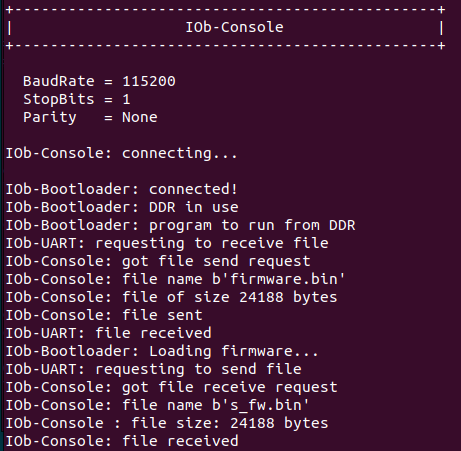
\includegraphics[width=\textwidth]{start_hello_fpga.png}
        \caption{Start of the \enquote{Hello World!} firmware.}
        \label{fig:start_hello_fpga}
    \end{subfigure}
    \hfill
    \begin{subfigure}[b]{0.49\textwidth}
        \centering
        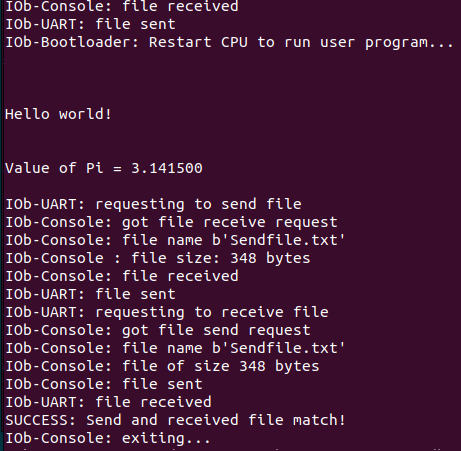
\includegraphics[width=\textwidth]{end_hello_fpga.png}
        \caption{End of the \enquote{Hello World!} firmware.}
        \label{fig:end_hello_fpga}
    \end{subfigure}
    \caption{Running the \enquote{Hello World!} firmware in the FPGA Board.}
    \label{fig:hello_fpga}
\end{figure}

The tables in \ref{tab:fpga_hello} are the FPGA implementation results for two FPGA families. The author implemented the developed \acrshort{soc} on the kintex Ultrascale AES-KU040-DB-G board and in the CYCLONE V GT-DK. The kintex Ultrascale has an \acrshort{fpga} more capable than the CYCLONE V.

\begin{table}[!ht]
    \begin{subtable}[h]{0.45\textwidth}
        \centering
        \begin{tabular}{l|l|l|}
            \cline{2-3}
                                              & \textit{IOb-SoC-Linux} & \textit{IOb-SoC} \\ \hline
            \multicolumn{1}{|l|}{ALM}         & 10,062                 & 9,280            \\ \hline
            \multicolumn{1}{|l|}{FF}          & 12150                  & 10020            \\ \hline
            \multicolumn{1}{|l|}{DSP}         & 8                      & 3                \\ \hline
            \multicolumn{1}{|l|}{BRAM blocks} & 234                    & 352              \\ \hline
            \multicolumn{1}{|l|}{BRAM bits}   & 753,248                & 779,744          \\ \hline
        \end{tabular}
       \caption{Cyclone V GT}
       \label{tab:cyclone_hello}
    \end{subtable}
    \hfill
    \begin{subtable}[h]{0.45\textwidth}
        \centering
        \begin{tabular}{l|l|l|}
            \cline{2-3}
                                            & \textit{IOb-SoC-Linux} & \textit{IOb-SoC} \\ \hline
            \multicolumn{1}{|l|}{LUTs}      & 21226                  & 23003            \\ \hline
            \multicolumn{1}{|l|}{Registers} & 23373                  & 22588            \\ \hline
            \multicolumn{1}{|l|}{DSPs}      & 10                     & 7                \\ \hline
            \multicolumn{1}{|l|}{BRAM}      & 39.5                   & 34.5             \\ \hline
        \end{tabular}
        \caption{Kintex Ultrascale}
        \label{tab:kintex_hello}
     \end{subtable}
     \caption{FPGA results for \enquote{Hello World!} program using external memory.}
     \label{tab:fpga_hello}
\end{table}

The author obtained the values in table \ref{tab:fpga_hello} while using the \acrshort{soc} with the external memory. When synthesising the \acrshort{soc}, the user can define whether he wants to use external memory with the \enquote{RUN\_EXTMEM} flag. If \enquote{RUN\_EXTMEM=1} then a memory controller will be synthesised alongside the developed \acrshort{soc} and loaded onto the \acrshort{fpga}. The memory controller is hardware logic written in Verilog and specific to the \acrshort{fpga} where the \acrshort{soc} is running. In order to better understand resource utilisation, the author decided to compare the resources used when running the \enquote{Hello World!} firmware from the internal memory. The resources without the memory controller are in tables \ref{tab:fpga_hello_int_mem}.

\begin{table}[!ht]
    \begin{subtable}[h]{0.45\textwidth}
        \centering
        \begin{tabular}{l|l|l|}
            \cline{2-3}
                                              & \textit{IOb-SoC-Linux} & \textit{IOb-SoC} \\ \hline
            \multicolumn{1}{|l|}{ALM}         & 3,687                  & 1,542            \\ \hline
            \multicolumn{1}{|l|}{FF}          & 4707                   & 1214             \\ \hline
            \multicolumn{1}{|l|}{DSP}         & 8                      & 3                \\ \hline
            \multicolumn{1}{|l|}{BRAM blocks} & 56                     & 38               \\ \hline
            \multicolumn{1}{|l|}{BRAM bits}   & 408,800                & 296,960          \\ \hline
        \end{tabular}
       \caption{Cyclone V GT}
       \label{tab:cyclone_hello_int_mem}
    \end{subtable}
    \hfill
    \begin{subtable}[h]{0.45\textwidth}
        \centering
        \begin{tabular}{l|l|l|}
            \cline{2-3}
                                            & \textit{IOb-SoC-Linux} & \textit{IOb-SoC} \\ \hline
            \multicolumn{1}{|l|}{LUTs}      & 5457                   & 2072             \\ \hline
            \multicolumn{1}{|l|}{Registers} & 4405                   & 1074             \\ \hline
            \multicolumn{1}{|l|}{DSPs}      & 7                      & 4                \\ \hline
            \multicolumn{1}{|l|}{BRAM}      & 14                     & 9                \\ \hline
        \end{tabular}
        \caption{Kintex Ultrascale}
        \label{tab:kintex_hello_int_mem}
     \end{subtable}
     \caption{FPGA results for \enquote{Hello World!} program.}
     \label{tab:fpga_hello_int_mem}
\end{table}

From the tables in \ref{tab:fpga_hello_int_mem} the author can confirm the \textit{VexRiscv} \acrshort{cpu} requires more resources than the \textit{PicoRV32}. Comparing tables \ref{tab:fpga_hello} and \ref{tab:fpga_hello_int_mem} the reader can see that there is a big difference in resources due to the utilization of the external memory. Interestingly, in table \ref{tab:cyclone_hello} the \textit{IOb-SoC-Linux} uses less \acrshort{bram}s than the \textit{IOb-SoC}. The \textit{IOb-SoC-Linux} uses less \acrshort{bram}s because the L1 cache integrated with the \textit{VexRiscv} \acrshort{cpu} is smaller than the L1 \textit{iob-cache} hardware module used by the \textit{IOb-SoC}. In table \ref{tab:fpga_hello_int_mem} the \textit{IOb-SoC-Linux} clearly uses more resources because the \textit{VexRiscv} \acrshort{cpu} contains the L1 cache and is more complex than the \textit{PicoRV32}. \textit{VexRiscv} is more complex than \textit{PicoRV32} because it supports more instruction extensions and has more \acrlong{csr}.

\section{Interrupt Routines}
\label{section:interrupt_routine}
To test the correct functionality of the interrupts in the \acrshort{soc}, the author executed the developed \acrshort{clint} testbench. Moreover, to test the complete \acrshort{soc}, he ran the bare-metal firmware created to handle interrupts. The firmware was executed in simulation and implemented in the \acrshort{fpga} Board.

The size of the firmware that tests the interrupt routine is 24364 Bytes. Consequently, the only difference in the \acrshort{soc} used on this section tests is the addition of the \acrshort{clint} hardware. The memory size is the same since the \enquote{Hello World!} program and this firmware have similar sizes, under 32 KB.

\subsection{Execute CLINT simulation}
After developing the \acrshort{clint} unit, the author executed its testbench, testing the timer and software interrupts. In figure \ref{fig:clint_sim} the readers can see a successful simulation of the \acrshort{clint} executing the interrupts.

\begin{figure}[!ht]
    \centering
    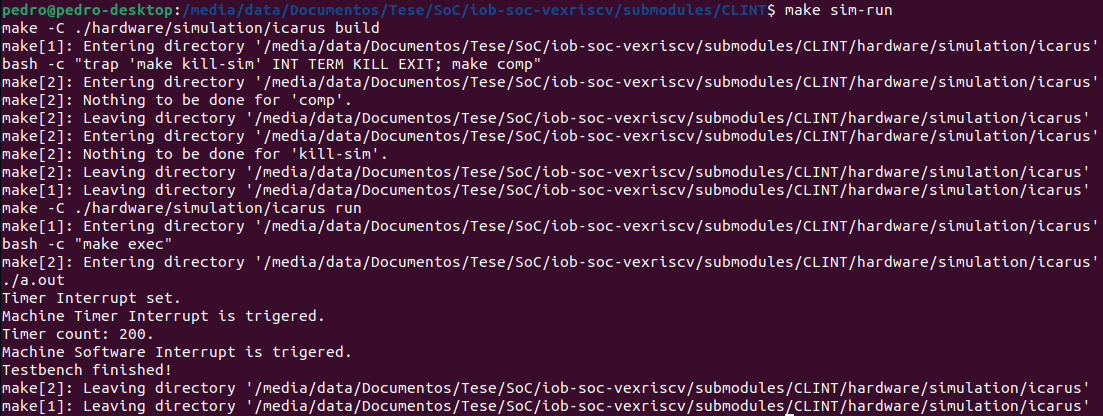
\includegraphics[width=\textwidth]{clint_sim.png}
    \caption{\acrshort{clint} timer and software interrupt simulation.}
    \label{fig:clint_sim}
\end{figure}

Explain all the simulation processes.

\subsection{Execute in simulation}
\begin{figure}[!ht]
    \centering
    \begin{subfigure}[b]{0.49\textwidth}
        \centering
        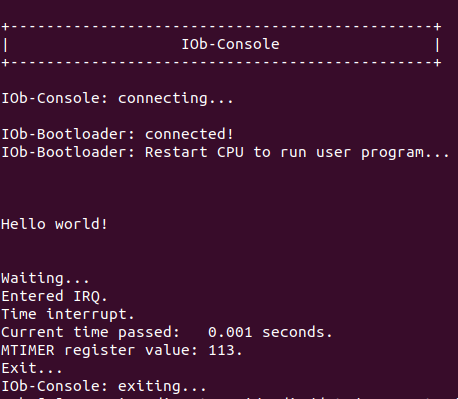
\includegraphics[width=\textwidth]{icarus_int_sim.png}
        \caption{Interrupt routine firmware with \textit{Icarus}.}
        \label{fig:icarus_int_sim}
    \end{subfigure}
    \hfill
    \begin{subfigure}[b]{0.49\textwidth}
        \centering
        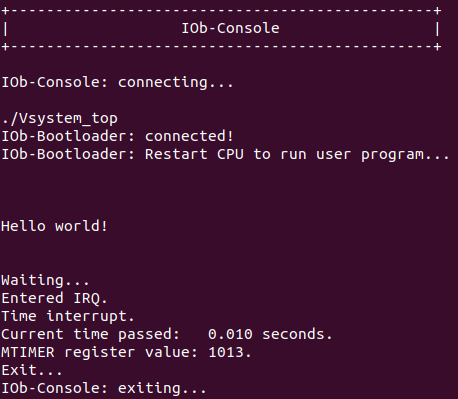
\includegraphics[width=\textwidth]{verilator_int_sim.png}
        \caption{Interrupt routine firmware with \textit{Verilator}.}
        \label{fig:verilator_int_sim}
    \end{subfigure}
    \caption{Running the interrupt routine firmware in the FPGA Board.}
    \label{fig:int_sim}
\end{figure}

\subsection{Execute in the FPGA Board}

\begin{figure}[!ht]
    \centering
    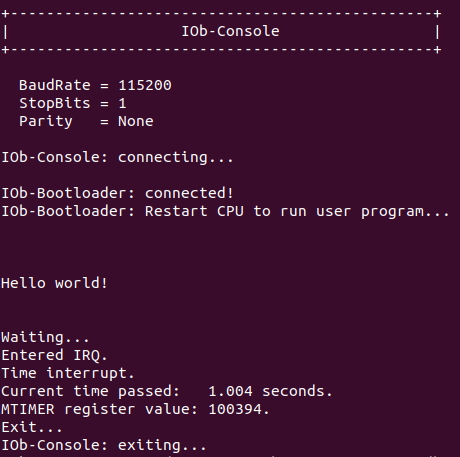
\includegraphics[width=0.49\textwidth]{int_fpga.png}
    \caption{Executing the interrupt routine program on the \acrshort{fpga}.}
    \label{fig:int_fpga}
\end{figure}
% talk 0.004 seconds after is time the interrupt handler takes to execute. It is different from the simulation because of the baud rate.

\begin{table}[!ht]
    \begin{subtable}[h]{0.45\textwidth}
        \centering
        \begin{tabular}{l|l|l|}
            \cline{2-3}
                                              & w/o DDR  & w/ DDR  \\ \hline
            \multicolumn{1}{|l|}{ALM}         & 3,883    & 10,257  \\ \hline
            \multicolumn{1}{|l|}{FF}          & 4940     & 12300   \\ \hline
            \multicolumn{1}{|l|}{DSP}         & 8        & 8       \\ \hline
            \multicolumn{1}{|l|}{BRAM blocks} & 56       & 234     \\ \hline
            \multicolumn{1}{|l|}{BRAM bits}   & 408,800  & 753,248 \\ \hline
        \end{tabular}
       \caption{Cyclone V GT}
       \label{tab:cyclone_int}
    \end{subtable}
    \hfill
    \begin{subtable}[h]{0.45\textwidth}
        \centering
        \begin{tabular}{l|l|l|}
            \cline{2-3}
                                            & w/o DDR  & w/ DDR \\ \hline
            \multicolumn{1}{|l|}{LUTs}      & 5729     & 21478  \\ \hline
            \multicolumn{1}{|l|}{Registers} & 4580     & 23545  \\ \hline
            \multicolumn{1}{|l|}{DSPs}      & 7        & 10     \\ \hline
            \multicolumn{1}{|l|}{BRAM}      & 14       & 39.5   \\ \hline
        \end{tabular}
        \caption{Kintex Ultrascale}
        \label{tab:kintex_int}
     \end{subtable}
     \caption{FPGA results for interrupt routine program.}
     \label{tab:fpga_int}
\end{table}


\section{Boot and use the Linux Operating System}
\label{section:boot_linux}
The objective of this thesis project was to run an \acrlong{os} in the \textit{IOb-SoC-Linux}. The \textit{IOb-SoC-Linux} used in this section adds the \acrshort{plic} hardware and substitutes the \textit{iob-UART} for the \textit{iob-UART16550}. The software that comprises the complete \acrshort{os} is the \textit{OpenSBI} bootloader, the \acrlong{dtb}, the Linux kernel and the \acrlong{rootfs}.

Table \ref{tab:time_os} presents how much time it takes to build the complete \acrshort{os} with the command \lstinline[language=sh]{make build-OS}. The \enquote{real} time is the time that passes since the user executes the command until it finishes. The \enquote{user} time is the time the \acrshort{cpu} takes while executing operations in the user space. The \enquote{user} time is bigger than the \enquote{real} time because it counts the time passed in each \acrshort{cpu} core. Part of the compilation of the \acrshort{rootfs} and the kernel is done in parallel using two cores.

\begin{table}[!ht]
    \centering
    \begin{tabular}{ll}
    real & 4m29,570s \\
    user & 8m12,039s \\
    sys  & 0m56,887s
    \end{tabular}
    \caption{Time it takes to build the \acrshort{os}.}
    \label{tab:time_os}
\end{table}

The \acrshort{os} size is to big to run in the \acrshort{fpga} internal memory. The \textit{OpenSBI} bootloader is 90896 Bytes. The \acrlong{dtb} is 1669 Bytes. The Linux kernel is 4426152 Bytes. Lastly the \acrlong{rootfs} is 1142733 Bytes. The memory has to have at least 8 MB ($2^23$) to store all this software. Consequently, the \textit{IOb-SoC-Linux} was tested and implemented on the \acrshort{fpga} with the external memory.

In figure \ref{fig:bootloader_sim} the reader can see the start of the \acrshort{os} simulation with \textit{Verilator}.

\begin{figure}[!ht]
    \centering
    \begin{subfigure}[b]{0.49\textwidth}
        \centering
        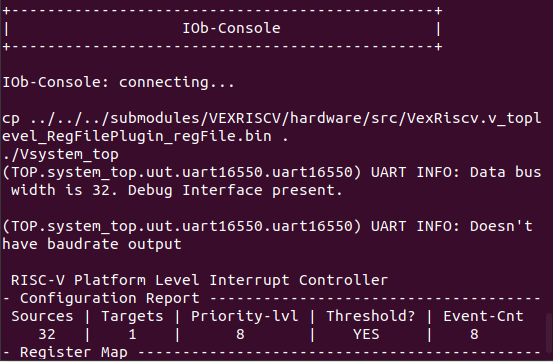
\includegraphics[width=\textwidth]{start_bootloader_sim.png}
        \caption{\textit{iob-UART16550} and \textit{iob-PLIC} properties.}
        \label{fig:start_bootloader_sim}
    \end{subfigure}
    \hfill
    \begin{subfigure}[b]{0.49\textwidth}
        \centering
        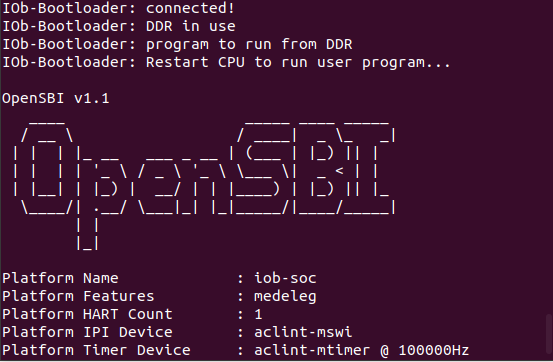
\includegraphics[width=\textwidth]{end_bootloader_sim.png}
        \caption{\textit{IOb-SoC} bootloader and \textit{OpenSBI} firmware.}
        \label{fig:end_bootloader_sim}
    \end{subfigure}
    \caption{Start of the \acrshort{os} simulation with \textit{Verilator}.}
    \label{fig:bootloader_sim}
\end{figure}

Figure \ref{fig:start_bootloader_sim} shows the initialization of the \textit{Console} program. Furthermore, it shows the instantiation of the \textit{iob-UART16550} and the \textit{iob-PLIC}. The \textit{iob-UART16550} and the \acrshort{plic} core have an initial block that prints their properties. The synthesis tools do not synthesise the initial block to real hardware, but the simulator executes it. Figure \ref{fig:end_bootloader_sim} shows the \textit{iob-bootloader} and the start of the \textit{OpenSBI} bootloader. The \textit{iob-bootloader} in figure \ref{fig:end_bootloader_sim} does not transfer the software to the memory because the author executed the simulation considering that the software was already in the memory.

Figure \ref{fig:start_linux_sim} shows the end of the \textit{OpenSBI} bootloader and the start of the Linux kernel. The first line printed by the Linux kernel indicates the author built the kernel executing, the kernel version and which toolchain he used to compile it.

\begin{figure}[!ht]
    \centering
    \centering
    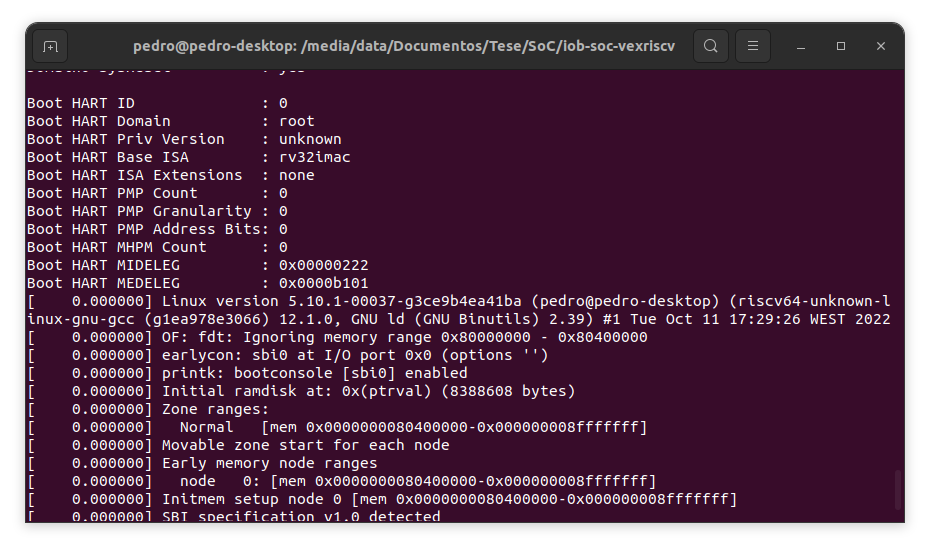
\includegraphics[width=0.9\textwidth]{start_Linux_sim.png}
    \caption{Start of the Linux kernel boot with \textit{Verilator}.}
    \label{fig:start_linux_sim}
\end{figure}

While figure \ref{fig:start_linux_sim} shows the start of the Linux kernel, figure \ref{fig:end_linux_verilator} shows the end of the Linux kernel booting process and the execution of the \enquote{init} script. The \enquote{init} script , as seen in subsection \ref{subection:linux_rootfs}, is the first program the \acrshort{os} executes after the Linux kernel mounts the \acrshort{rootfs} and finishes booting. There exist multiple messages printed to the terminal between the output shown in figure \ref{fig:start_linux_sim} and in \ref{fig:end_linux_verilator}. Those messages show the progress while the Linux kernel boots. The Linux kernel boot process's last message is \lstinline{Run /init as init process}. After that message the \acrshort{soc} executes the \enquote{init} program.

\begin{figure}[!ht]
    \centering
    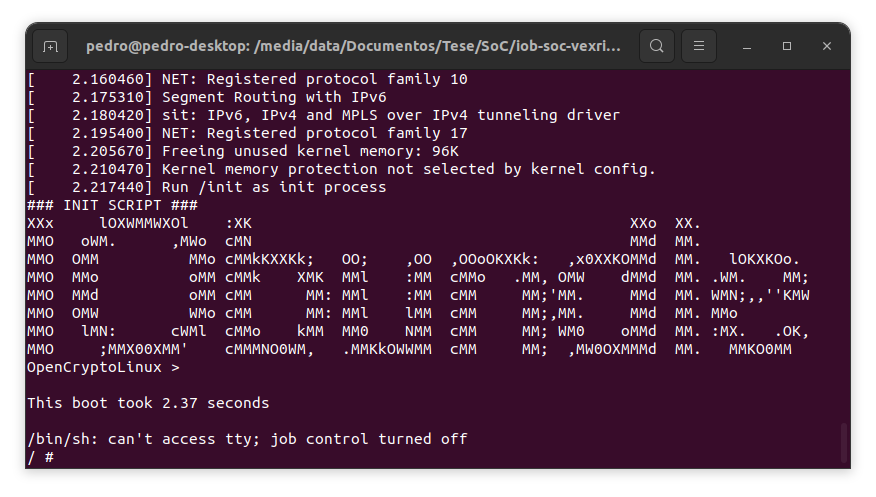
\includegraphics[width=0.9\textwidth]{end_Linux_sim.png}
    \caption{End of Linux kernel boot with \textit{Verilator}.}
    \label{fig:end_linux_verilator}
\end{figure}

The warning \lstinline{/bin/sh: can't access tty; job control turned off} that appears at the end of the Linux boot in figure \ref{fig:end_linux_verilator} means the shell program is not writing to a \textit{tty}, but a socket. Advanced commands such as Ctrl+Z and Ctrl+C are unavailable when writing to a socket. Furthermore, sh will not support background processes (command \&) and the associated bg/fg/disown/jobs commands. However, processes forking themselves and closing their inputs will still work. This way, the system is protected from a race condition that could occur if both the shell and the background process were waiting for user input. This problem happens because the author developed the \acrshort{rootfs} to be lightweight for embedded systems. Consequently, it does not implement some Linux files and programs that would enable such features. The \enquote{init} script could call the shell program could with \lstinline[language=sh]{sh +m}.

Figure \ref{fig:linux_fpga} shows the developed minimal \acrshort{os} running on an \acrshort{fpga}. The reader can see that the author has suppressed the shell warning. The initial part of the figure shows the final stage of the Linux kernel booting. After booting, the author tested the \lstinline[language=sh]{ls /} command that showed the files and directories in the systems' root. Lastly the author executed the \lstinline[language=sh]{cat init} command for the \acrshort{os} to print the contents of the \enquote{init} script to the terminal. The difference between the \enquote{init} script printed and the one presented in listing \ref{lst:rootfs_init} is that \enquote{IObundle} is printed as a design with \acrshort{ascii} characters and the shell program is called with the \enquote{+m} argument.

\begin{figure}[!ht]
    \centering
    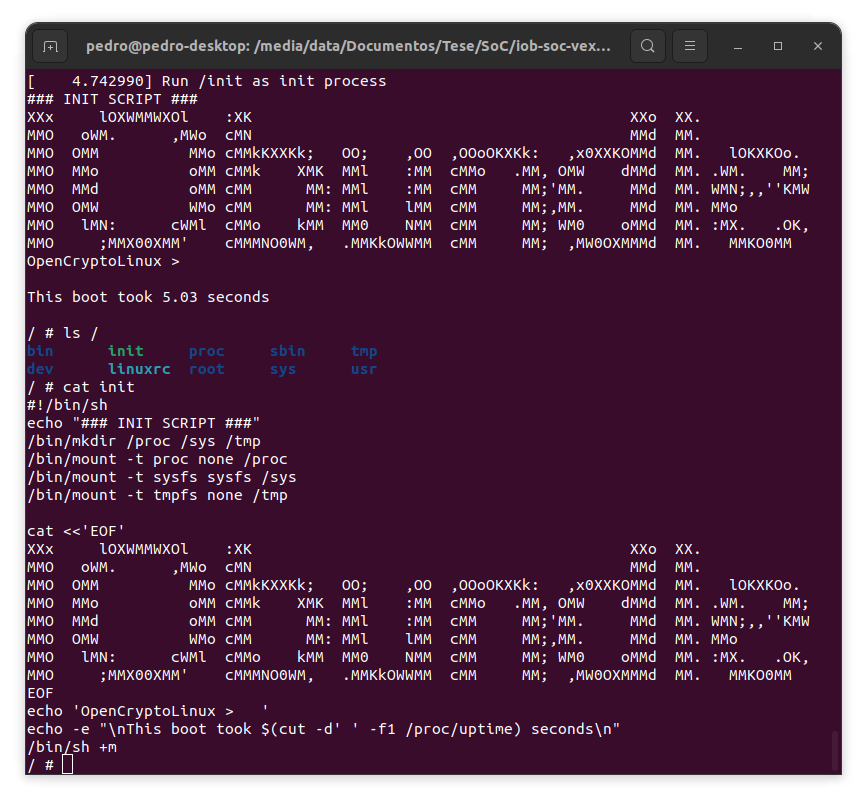
\includegraphics[width=0.9\textwidth]{linux_fpga.png}
    \caption{Linux kernel boot in the \acrshort{fpga}.}
    \label{fig:linux_fpga}
\end{figure}

The time the Linux kernel takes to boot in real hardware, figure \ref{fig:linux_fpga}, is almost double what it takes to boot in simulation, figure \ref{fig:linux_fpga}. The time to boot is almost double because the memory module used in the simulation does not have any latency. When the L2 cache fetches data from memory in real hardware, it must wait before receiving the data burst. Using the \textit{CYCLONE V} \acrshort{fpga} board the Linux kernel takes 7.01 seconds to boot. The author expected the boot to take longer since the system clock frequency used with the \textit{CYCLONE V} is 50 MHz. The Kintex Ultrascale was able to run with a frequency of 100 MHz. The \textit{OpenSBI} bootloader and the \acrlong{dtb} had to be recompiled with the system frequency defined to 50 MHz.

Table \ref{tab:fpga_linux} show the resources used by the \textit{IOb-SoC-Linux} in the different \acrshort{fpga}s.

\begin{table}[!ht]
    \begin{subtable}[h]{0.45\textwidth}
        \centering
        \begin{tabular}{l|l|l|}
            \hline
            \multicolumn{1}{|l|}{ALM}         & 11,227  \\ \hline
            \multicolumn{1}{|l|}{FF}          & 13725   \\ \hline
            \multicolumn{1}{|l|}{DSP}         & 8       \\ \hline
            \multicolumn{1}{|l|}{BRAM blocks} & 234     \\ \hline
            \multicolumn{1}{|l|}{BRAM bits}   & 755,424 \\ \hline
        \end{tabular}
       \caption{Cyclone V GT}
       \label{tab:cyclone_linux}
    \end{subtable}
    \hfill
    \begin{subtable}[h]{0.45\textwidth}
        \centering
        \begin{tabular}{l|l|l|}
            \hline
            \multicolumn{1}{|l|}{LUTs}      & 23126 \\ \hline
            \multicolumn{1}{|l|}{Registers} & 24505 \\ \hline
            \multicolumn{1}{|l|}{DSPs}      & 10    \\ \hline
            \multicolumn{1}{|l|}{BRAM}      & 39.5  \\ \hline
        \end{tabular}
        \caption{Kintex Ultrascale}
        \label{tab:kintex_linux}
     \end{subtable}
     \caption{FPGA results for interrupt routine program.}
     \label{tab:fpga_linux}
\end{table}

The difference in registers between tables. MABE is not sure if there is space.
